\subsection{Klasyfikacja podatności}
Ryzyko związane z podatnościami zostało wyznaczone na podstawie powagi konsekwencji ich nadużycia oraz trudności wykorzystania ich do ataku. Wyznaczone zostało 5 klas:
\begin{itemize}
    \item \colorbox{red!80}{WYSOKIE} - zawiera najpoważniejsze podatności pozwalające na ataki, które naruszają bezpieczeństwo użytkowników i/lub sprawność aplikacji. Ich obecność oznacza, że działanie aplikacji powinno zostać niezwłocznie wstrzymane w celu poprawy zabezpieczeń
    \item \colorbox{orange!80}{ŚREDNIE} - zawiera podatności, które mają poważne, ale nie krytyczne skutki lub pozwalają na szybkie i łatwe zakłócenie pracy aplikacji. Nie wymagają one wyłączania aplikacji, ale powinny zostać dopisane na listę zadań o wysokim priorytecie
    \item \colorbox{yellow!80}{NISKIE} - pozostałe podatności, czyli te których skutki nie są zbyt poważne lub szansa na ich wykonanie bez dodatkowej wiedzy o systemie jest praktycznie niemożliwe
    \item \colorbox{green!80}{BEZPIECZNE} - dodatkowa kategoria przedstawiające podatności, które były badane ale nie udało się udowodnić, że istnieją i można je wykorzystać. Ta klasa została dodana ze względu na wymagania kursu i służy do przedstawienia wszystkich wykonanych badań. Z powodu, że takie podatności były badane znacznie szerzej opisy zawarte w tej klasie są luźniejsze i bardziej opisowe (w stylu sprawozdania, nie do końca raportu)
    \item \colorbox{cyan}{INFORMACYJNE} - zawiera dodatkowe zalecenia i propozycje poprawek
\end{itemize}
Podział klas ze względu na prawdopodobieństwo wykonania ataku i powagi jego konsekwencji został zaprezentowany w formie wizualnej na rysunku \ref{img:tab}. 

\begin{figure}[H]
\caption{Tabela prezentująca podział klas ryzyka podatności ze względu na oceny prawdopodobieństwo nadużycia i powagi potencjalnych skutków}
\label{img:tab}
\centering
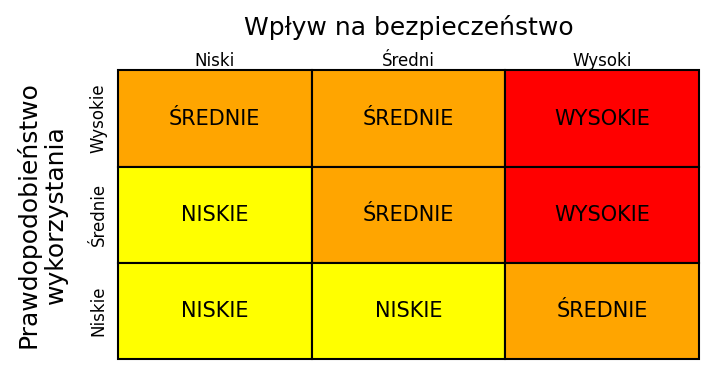
\includegraphics[width=0.9\textwidth]{img/tab.png}
\end{figure}

W trakcie analizy raportu należy pamiętać, że zarówno definicja klas, jak i sama ocena prawdopodobieństwa i powagi podatności jest \textbf{subiektywna}!

\subsection{Znalezione podatności}
Liczba znalezionych niedoskonałości ze względu na przypisaną im klasę ryzyka została przedstawiona na rysunku \ref{img:stat}.

\begin{figure}[H]
\caption{Rozkład znalezionych podatności według ich klasyfikacji}
\label{img:stat}
\centering

\includegraphics[width=\textwidth]{img/bars.png}
\end{figure}

Można zaobserwować, że występują liczne zagrożenia o wysokim i średnim ryzyku, dlatego w celu poprawy bezpieczeństwa \newline\huge\color{red}{\textbf{działanie aplikacji powinno zostać jak najszybciej wstrzymane}} \normalsize\normalcolor

W tabeli \ref{tab:podsumowanie} zawarto podsumowanie przeprowadzonych badań. Każda podatność posiada swój kod, skrócony opis słowny oraz przypisane klasy ryzyka, prawdopodobieństwa i wpływu na bezpieczeństwo wraz z krótkim uzasadnieniem podjętej decyzji.

%\Huge
%\centering
%\resizebox{1.05\columnwidth}{!}{%

% Please add the following required packages to your document preamble:
% \usepackage[table,xcdraw]{xcolor}
% Beamer presentation requires \usepackage{colortbl} instead of \usepackage[table,xcdraw]{xcolor}
\begin{table}[H]
\caption{Tabela podsumowująca podatności i ryzyka z nimi związane}
\label{tab:podsumowanie}

\Huge
\centering
\resizebox{1.05\columnwidth}{!}{%
\begin{tabular}{|l|l|c|l|l|}
\hline
\rowcolor[HTML]{EFEFEF} 
\multicolumn{1}{|c|}{\cellcolor[HTML]{EFEFEF}\textit{Kod podatności}} & \multicolumn{1}{c|}{\cellcolor[HTML]{EFEFEF}\textit{Nazwa}}                                                             & \textit{Klasa ryzyka}                                                                        & \multicolumn{1}{c|}{\cellcolor[HTML]{EFEFEF}\textit{\begin{tabular}[c]{@{}c@{}}Prawdopodobieństwo\\ wykonania\end{tabular}}}                                                                                        & \multicolumn{1}{c|}{\cellcolor[HTML]{EFEFEF}\textit{\begin{tabular}[c]{@{}c@{}}Wpływ na \\ bezpieczeństwo\end{tabular}}}                           \\ \hline
PT01-DICT                                                             & Atak słownikowy                                                                                                         & \cellcolor[HTML]{FE0000}{\color[HTML]{000000} \textbf{WYSOKIE}}                              & \begin{tabular}[c]{@{}l@{}}ŚREDNIE (brak jakichkolwiek \\ zabezpieczeń, atak jest trywialny w \\ wykonaniu i oczywisty, z drugiej strony \\ użytkownicy często dbają sami o siebie \\ długimi hasłami)\end{tabular} & \begin{tabular}[c]{@{}l@{}}WYSOKI (pełen dostęp do \\ zaatakowanego konta)\end{tabular}                                                            \\ \hline
PT02-SQL-INJ                                                          & \begin{tabular}[c]{@{}l@{}}Wydobycie haseł użytk.\\ z użyciem klasycznego \\ SQL Injection\end{tabular}                 & \cellcolor[HTML]{FE0000}{\color[HTML]{333333} \textbf{WYSOKIE}}                              & \begin{tabular}[c]{@{}l@{}}WYSOKIE (jeden z bardziej oczywistych\\ łatwych ataków, brak zabezpieczeń)\end{tabular}                                                                                                  & \begin{tabular}[c]{@{}l@{}}WYSOKI (dostęp do całej \\ bazy danych, w tym haseł \\ w postaci przestarzałego hasha\\ md5)\end{tabular}               \\ \hline
\begin{tabular}[c]{@{}l@{}}PT03-BLD-SQL\\ -INJ\end{tabular}           & \begin{tabular}[c]{@{}l@{}}Wydobycie hasha hasła \\ wybranego użytkownika \\ z użyciem Blind SQL Injection\end{tabular} & \cellcolor[HTML]{FE0000}\textbf{WYSOKIE}                                                     & \begin{tabular}[c]{@{}l@{}}ŚREDNIE (mało popularny atak, opiera się o\\ użycie podatności PT02, która jest znacznie\\ bardziej wartościowa)\end{tabular}                                                            & \begin{tabular}[c]{@{}l@{}}WYSOKI (dostęp do niskiej \\ jakości hasha hasła użytkownika)\end{tabular}                                              \\ \hline
\begin{tabular}[c]{@{}l@{}}PT04-NO-SQL\\ -INJ\end{tabular}            & \begin{tabular}[c]{@{}l@{}}Masowa modyfikacja opinii \\ z użyciem NoSQL Injection\end{tabular}                          & \cellcolor[HTML]{FFC702}\textbf{ŚREDNIE}                                                     & \begin{tabular}[c]{@{}l@{}}NISKIE (atakujący musi wiedzieć o użyciu\\ bazy NoSQL)\end{tabular}                                                                                                                      & \begin{tabular}[c]{@{}l@{}}WYSOKI (możliwość modyfikacji \\ wszystkich danych w tabeli równoznaczne\\ z jej zniszczeniem)\end{tabular}             \\ \hline
PT05-RFL-XSS                                                          & \begin{tabular}[c]{@{}l@{}}Kradzież ciasteczek z użyciem\\ Reflected XSS\end{tabular}                                   & \cellcolor[HTML]{FFC702}\textbf{ŚREDNIE}                                                     & \begin{tabular}[c]{@{}l@{}}NISKIE (użytkownik musi kliknąć \\ w podejrzany link od atakującego)\end{tabular}                                                                                                        & \begin{tabular}[c]{@{}l@{}}WYSOKI (uzyskanie pełnego dostępu do\\ konta ofiary)\end{tabular}                                                       \\ \hline
PT06-CSP                                                              & \begin{tabular}[c]{@{}l@{}}Wymuszenie zmiany \\ polityki CSP\end{tabular}                                               & \cellcolor[HTML]{FCFF2F}\textbf{NISKIE}                                                      & \begin{tabular}[c]{@{}l@{}}NISKIE (wymaga żetonu pozwalającego\\ na zmianę awatara użytkownika,\\ awatar występuje tylko na\\ stronie profilu)\end{tabular}                                                         & \begin{tabular}[c]{@{}l@{}}NISKIE (sam w sobie nic nie robi, ale\\ pozwala na potencjalne wykonanie XSS \\ na użytkowniku)\end{tabular}            \\ \hline
PT07-XSS                                                              & Prosty atak Stored XSS                                                                                                  & \cellcolor[HTML]{34FF34}\textbf{BEZPIECZNE}                                                  & \begin{tabular}[c]{@{}l@{}}BRAK (sanityzacja nie pozwoliła na \\ wykonanie XSS metodą bezpośrednią)\end{tabular}                                                                                                    & -                                                                                                                                                  \\ \hline
PT08-SQL-XSS                                                          & \begin{tabular}[c]{@{}l@{}}Atak Stored XSS wspierany \\ przez SQL Injection\end{tabular}                                & \cellcolor[HTML]{34FF34}\textbf{BEZPIECZNE}                                                  & \begin{tabular}[c]{@{}l@{}}BRAK (mimo braku sanityzacji \\ nie udało się dodać nowych \\ danych do bazy SQL)\end{tabular}                                                                                           & -                                                                                                                                                  \\ \hline
PT09-RCE-XSS                                                          & \begin{tabular}[c]{@{}l@{}}Atak Stored XSS wspierany \\ przez RCE\end{tabular}                                          & \cellcolor[HTML]{FFC702}\textbf{ŚREDNIE}                                                     & \begin{tabular}[c]{@{}l@{}}NISKIE (atakujący musi posiadać dostęp do \\ zmiany pseudonimu użytkownika oraz wykonać\\ skuteczny atak PT06-CSP)\end{tabular}                                                          & \begin{tabular}[c]{@{}l@{}}ŚREDNI (pozwala wykonać \\ dowolny atak XSS tylko na \\ wybranego użytkownika)\end{tabular}                             \\ \hline
PT10-RCE                                                              & \begin{tabular}[c]{@{}l@{}}Kradzież danych z serwera\\ z użyciem RCE na szablonie\end{tabular}                          & \cellcolor[HTML]{FE0000}\textbf{WYSOKIE}                                                     & \begin{tabular}[c]{@{}l@{}}WYSOKIE (bardzo prosty atak, choć wymaga\\ wiedzy o użytej do generacji stron bibliotece)\end{tabular}                                                                                   & \begin{tabular}[c]{@{}l@{}}WYSOKI (pełen dostęp do \\ wnętrza kontenera)\end{tabular}                                                              \\ \hline
\begin{tabular}[c]{@{}l@{}}PT11-NOSQL\\ -RCE\end{tabular}             & \begin{tabular}[c]{@{}l@{}}Atak RCE z użyciem bazy \\ NoSQL\end{tabular}                                                & \cellcolor[HTML]{FCFF2F}\textbf{NISKIE}                                                      & \begin{tabular}[c]{@{}l@{}}ŚREDNIE (prosty atak, ale wymaga wiedzy o\\ użyciu bazy NoSQL)\end{tabular}                                                                                                              & \begin{tabular}[c]{@{}l@{}}NISKI (ograniczony kontekst zapytań nie\\ pozwala na zbyt wiele, jednym z zastosowań\\ może być atak SSRF)\end{tabular} \\ \hline
PT12-PTH-TRV                                                          & Atak Path Traversal                                                                                                     & \cellcolor[HTML]{34FF34}\textbf{BEZPIECZNE}                                                  & \begin{tabular}[c]{@{}l@{}}BRAK (końcówka ftp nigdy nie zwróciła pliku\\ spoza dozwolonego katalogu)\end{tabular}                                                                                                   & -                                                                                                                                                  \\ \hline
PT13-NL-BT                                                            & Atak Null Byte Poisoning                                                                                                & \cellcolor[HTML]{F8FF00}\textbf{NISKIE}                                                      & \begin{tabular}[c]{@{}l@{}}NISKIE (wymaga wiedzy o ukrytej\\ końcówce oraz potrzebie podwójnego\\ zakodowania null byte'a)\end{tabular}                                                                             & \begin{tabular}[c]{@{}l@{}}NISKI (dostęp do plików \\ serwowanych na końcówce)\end{tabular}                                                        \\ \hline
\begin{tabular}[c]{@{}l@{}}PT14-NL-BT\\ -PTH-TRV\end{tabular}         & \begin{tabular}[c]{@{}l@{}}Atak Path Traversal z \\ użyciemNull Byte Poisoning\end{tabular}                             & \cellcolor[HTML]{38FFF8}\textbf{\begin{tabular}[c]{@{}c@{}}BEZPIECZNE\\ / INFO\end{tabular}} & \begin{tabular}[c]{@{}l@{}}NISKIE (wymaga wiedzy o ukrytej\\ końcówce oraz potrzebie podwójnego\\ zakodowania null byte'a)\end{tabular}                                                                             & \begin{tabular}[c]{@{}l@{}}BRAK (ale zwracane błędy sugerują, że \\ przetwarzanie może nie być w pełni\\ bezpieczne)\end{tabular}                  \\ \hline
PT15-UN-AC                                                            & \begin{tabular}[c]{@{}l@{}}Nieautoryzowany dostęp \\ do danych\end{tabular}                                             & \cellcolor[HTML]{FFC702}\textbf{ŚREDNIE}                                                     & \begin{tabular}[c]{@{}l@{}}ŚREDNIE (łatwe w wykonaniu, ale używa \\ nieoczywistej końcówki)\end{tabular}                                                                                                            & \begin{tabular}[c]{@{}l@{}}ŚREDNI (podglądanie koszyka to \\ naruszenie prywatności, ale nie \\ bezpieczeństwa)\end{tabular}                       \\ \hline
PT16-SSRF                                                             & Atak Server Side Request Forgery                                                                                        & \cellcolor[HTML]{FFCB2F}\textbf{ŚREDNIE}                                                     & WYSOKIE (banalne wykonanie)                                                                                                                                                                                         & \begin{tabular}[c]{@{}l@{}}ŚREDNI (możliwość rekonesansu \\ sieci wewnętrznej lub użycia \\ sklepu jako pośrednika)\end{tabular}                   \\ \hline
PT17-CSRF                                                             & Atak Cross-Site Request Forgery                                                                                         & \cellcolor[HTML]{FFCB2F}\textbf{ŚREDNIE}                                                     & \begin{tabular}[c]{@{}l@{}}NISKIE (nowoczesne przeglądarki \\ pomagają z tego typu atakami mimo \\ braku zabezpieczeń w aplikacji)\end{tabular}                                                                     & \begin{tabular}[c]{@{}l@{}}WYSOKI (możliwość wykonania \\ dowolnej akcji w imieniu użytkownika)\end{tabular}                                       \\ \hline
PT18-JWT-NONE                                                         & \begin{tabular}[c]{@{}l@{}}Użycie niepodpisanego \\ żetona JWT\end{tabular}                                             & \cellcolor[HTML]{34FF34}\textbf{BEZPIECZNE}                                                  & \begin{tabular}[c]{@{}l@{}}BRAK (tak zmodyfikowane żetony \\ są automatycznie odrzucane)\end{tabular}                                                                                                               & -                                                                                                                                                  \\ \hline
PT19-JWT-HS                                                           & \begin{tabular}[c]{@{}l@{}}Użycie żetona JWT z innym \\ algorytmem podpisu\end{tabular}                                 & \cellcolor[HTML]{34FF34}\textbf{BEZPIECZNE}                                                  & \begin{tabular}[c]{@{}l@{}}BRAK (zmodyfikowany żeton jest blokowany \\ przez wszystkie sprawdzone końcówki)\end{tabular}                                                                                            & -                                                                                                                                                  \\ \hline
PT20-FAIL                                                             & \begin{tabular}[c]{@{}l@{}}Awaria serwera powodowana\\ uczciwymi akcjami\end{tabular}                                   & \cellcolor[HTML]{FE0000}\textbf{WYSOKIE}                                                     & \begin{tabular}[c]{@{}l@{}}WYSOKIE (wywoływane przez przypadek \\ podczas korzystania z podstawowych \\ funkcji aplikacji)\end{tabular}                                                                             & \begin{tabular}[c]{@{}l@{}}WYSOKI (doprowadza do awarii \\ serwera oraz wyczyszczenia baz danych)\end{tabular}                                     \\ \hline
\end{tabular}
}
\end{table}